\chapter{Introduction}
\label{ch:Intro}
\par
The unifying theme in this thesis is the presence of hidden hyperbolic geometries in strongly interacting systems and their bilayers. 

What is a fermi liquid? and what is a non-fermi liquid 

Consider a scattering diagram: self energy proportional to DoS, van hove points can break fermi liquid theory. cite polchinski, shankar.

\newpage     

\section{Interactions enhanced by van hove singularities}


\section{Graphene and its bilayers}
\label{sec:graphene}
Graphene is a single sheet of carbon atoms arranged in a hexagonal lattice~\cite{neto2009electronic}. Its electronic properties can be described by a simple tight binding model which accounts for electrons hopping between nearest neighbors in its two sublattices, with its hamiltonian given by
\begin{align}
    H &= -t \sum_{\langle i,j\rangle} a_i^\dagger b_j + h.c ,  
\end{align}
and can be diagonalized in terms of two component wavefunctions 
\begin{align}
    \Psi_i = \mqty(a_i \\ b_i  ) .
\end{align}
to obtain a spectrum given by 
\begin{align}
    E(\Vec{k}) &= \pm \sqrt{1 + 4\cos{\left(\frac{3 k_x a}{2}\right)}\cos{\left(\frac{\sqrt{3}k_y a}{2}\right)} + 4\cos^2{\left(\frac{\sqrt{3}k_y a}{2}\right)}}
    \label{eq:Graphene dispersion}
\end{align}

\begin{figure}[]
	\centering
	\begin{subfigure}{0.5\linewidth}
		\centering
		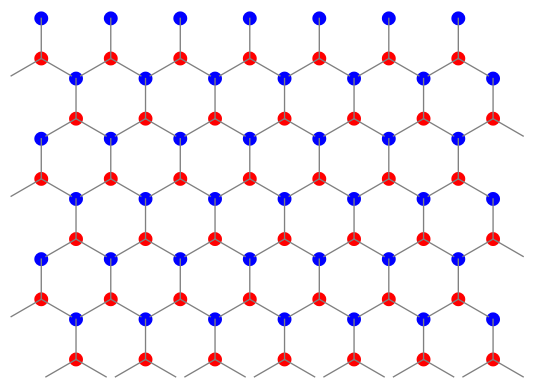
\includegraphics[width=4cm]{figures/introduction/graphene lattice.png}
            \caption{\centering}
	\end{subfigure}%
        \begin{subfigure}{0.5\linewidth}
		\centering
		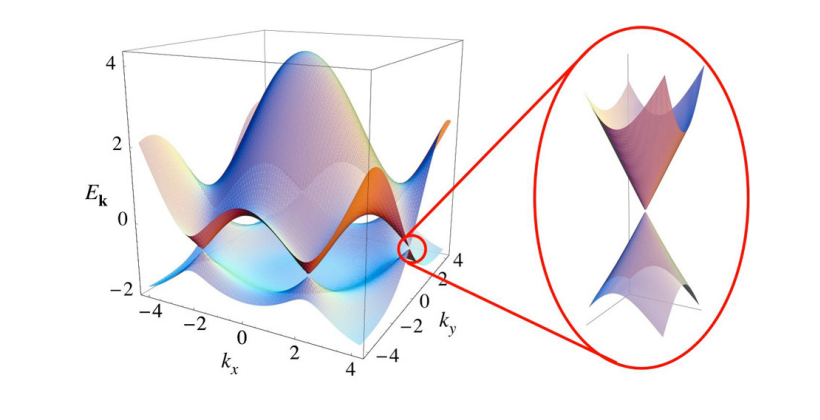
\includegraphics[width=5cm]{figures/introduction/bandstructure_graphene.png}
            \caption{\centering}
	\end{subfigure}%
	
 	\centering
	\begin{subfigure}{0.45\linewidth}
		\centering
		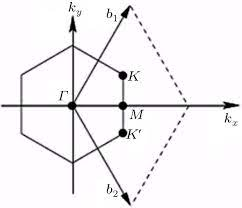
\includegraphics[width=4cm]{figures/introduction/brilluoinzonegraphene.png}
            \caption{\centering}
	\end{subfigure}
	\begin{subfigure}{0.45\linewidth}
		\centering
		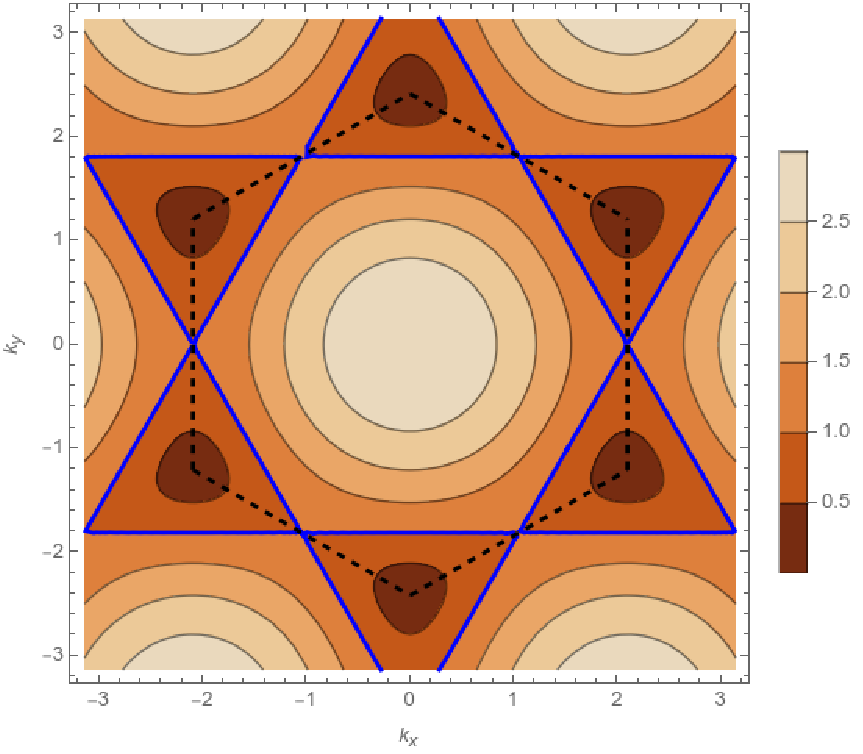
\includegraphics[width=4cm]{figures/introduction/graphenecontours.pdf}
            \caption{\centering}
	\end{subfigure}

	\caption{(a) Schematic hexagonal lattice of graphene showing carbon atoms in the A(red) and B(blue) sublattices. (b) Dispersion with zoom near the band-touching Dirac point. (c) The corresponding Brillouin zone marking the positions of the high symmetry points. (d) Energy contours of graphene showing the brilluoin zone in black dashed lines. The highlighted contour in blue is at the van Hove energy. (panels (b) and (c) taken from \cite{neto2009electronic}).}
	\label{fig:grapheneschematic}
\end{figure}

The dispersion in Eq.~\eqref{eq:Graphene dispersion} shows interesting features at the $K, K^\prime$ and the $M$ points of the Brilluoin zone. 

\par
The $K$ point and its time reversed partner $K^\prime$ points are referred to as Dirac points. This is because the gap between the two bands closes at these points, and the dispersion is linear. Indeed, the low energy hamiltonian close to for momenta $\vec{p}$ close to the $K$ point can be represented as 
\begin{align}
    H = v_F \,\Vec{p} \cdot \Vec{\sigma}.
    \label{eq:DiracHam}
\end{align}
\par 
The Dirac matrices in two dimensions are simply the $2x2$ Pauli matrices given by $\vec{\sigma}$. 
The corresponding dispersion $E(\Vec{p}) = v_F \abs{\vec{p}}$ is dubbed a Dirac cone, because it looks like a causal light cone from special relativity, just with an effective speed of light $v_F$. 

\par 
Graphene also has an interesting saddle-like dispersion near its $M$ point. This is shown in panels (b) and (d) of Fig.\ref{fig:grapheneschematic}. 








\section{The Kondo effect}
\section{The Sachdev-Ye-Kitaev model}


\section{This thesis}
In the introduction, we have covered the basic ideas used later in this thesis. We started with introductory topics in thermodynamics and statistical physics, then moved to a basic introduction to Monte Carlo methods and all the required knowledge to understand our physical system's simulation design and analyze the results. The proceeding section was dedicated to the basics of machine learning, deep learning, and appropriate selection of model, loss function, and minimization method. The last section culminated in a synergy of the previously mentioned topics by combining quantum physics, Monte Carlo methods, and neural networks in neural quantum states that we used to find the ground state and its energy of lattice gauge theories.

\subsection{Chapter 1 - The Kondo effect in Twisted bilayer graphene}


\subsection{Chapter 2 - Chaos in the bipartite Sachdev-Ye-Kitaev model}



\subsection{Chapter 3 - Wormholes in the Yukawa-Sachdev-Ye-Kitaev model}

